\documentclass{beamer}
\usepackage[utf8x]{inputenc}
\usepackage[ngerman]{babel}	
\setbeamertemplate{navigation symbols}{}


\title{Handbuch JerusalemDB}
\author{Hanno Wierichs}
\institute{}
\date{\today}

 \begin{document}
	\begin{frame}[plain]
		\titlepage
	\end{frame}

	\begin{frame}{Inhaltsverzeichnis}
		\tableofcontents
	\end{frame} 


\section{Problem} 
		\begin{frame}
			\frametitle{Problem}
			Beispiel Ort "'Haus der Maria"'
					\begin{itemize}
						\item Quelle A, 16. Jh.: "'Haus der Maria, 60 Doppelschritte nördlich des Tempelbergs, nicht unmittelbar neben der Stadtmauer"'
						\item Quelle B, 16. Jh.: "'Ort an dem Maria geboren wurde, 20 Doppelschritte nordwestlich des Löwentors, 20 Schritte westlich der Stadtmauer"'
						\item Quelle C, 19. Jh.: "'Marias Geburtsstätte, zwischen Österreichischem Hospiz und Stadtmauer"'
					\end{itemize}					 
					\vspace{1ex}
					\begin{itemize}
						\item[$\Rightarrow$] Orte können zeitabhängig verschiedene Bezeichner haben
						\item[$\Rightarrow$] Orte können zeitabhängig verschiedene Lokalisierungen haben
						\item[$\Rightarrow$] Orte können nicht durchgängig punktuell lokalisiert werden	
					\end{itemize}					 					
	\end{frame}
	
	
\section{Lösung} 
\begin{frame}
			\frametitle{Lösung}
			\begin{columns}
			\column{0.6\textwidth}
			\begin{itemize}
				\item Topos
					\begin{itemize}
						\item Name
					\end{itemize} 
					\item Place
					\begin{itemize}
						\item Name
						\item punktuell lokalisiert
						\item zeitliche Gültigkeit 												
						\item optional: additional instances
					\end{itemize}
					\item Topos $\Leftrightarrow$ Place beliebig
					\begin{itemize}
						\item optional: zeitliche Gültigkeit für Verknüpfung
					\end{itemize}
			\end{itemize}
			\column{0.4\textwidth}
					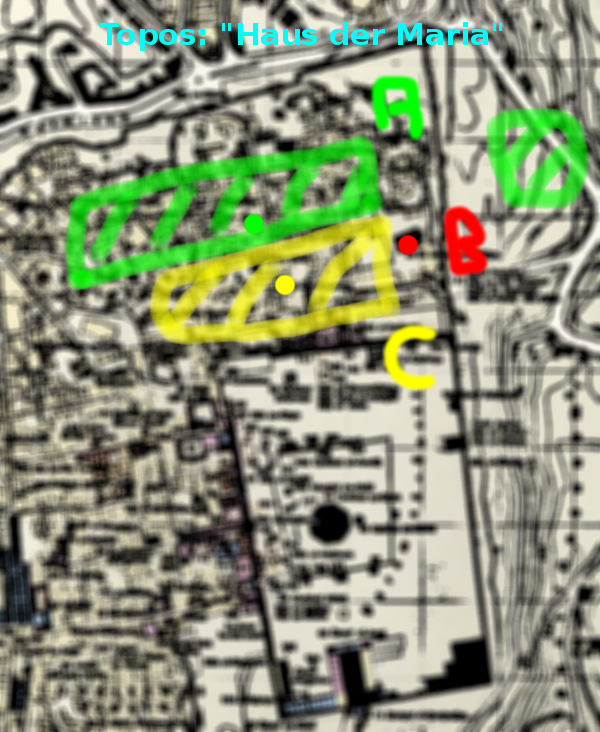
\includegraphics[width=\linewidth]{detail_1}
			\end{columns}
	\end{frame}

	\begin{frame}
			\frametitle{Lösung}
			\begin{itemize}
				\item ein Dokument - viele Einträge
				\item ein Eintrag - viele Topos\_in\_Eintrag
				\item Topos\_in\_Eintrag: 
				\begin{itemize}
					\item Eintrag $\Leftrightarrow$ Topos 
					\item optional: Eintrag $\Leftrightarrow$ Place 
					\item optional: alternativer Name für Topos
					\item optional: Sortierungszahl
				\end{itemize}			 
			\end{itemize} 		
	\end{frame}

	\begin{frame}
			\frametitle{Lösung}
			\begin{itemize}
  					\item relationale Modellierung:
					\begin{itemize}
						\item unabhängige Entities: Autor, Dokument,Topos, Place
						\item abhängige Entities: Eintrag,Topos\_in\_Eintrag, Placetopos
					\end{itemize}
				\end{itemize} 
	\end{frame}
	
	\begin{frame}
			\frametitle{Lösung - Modellierung [schematische Darstellung]} 
				\begin{figure}
					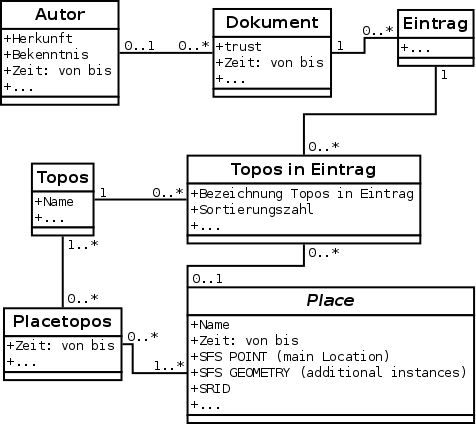
\includegraphics[scale=0.3]{detail_2.png} 
				\end{figure}			
	\end{frame}

\section{Software}	
\begin{frame}
			\frametitle{Software - Installation} 
				\begin{itemize}
					\item JerusalemDB.jar installiert erforderliche Strukturen und dient als Programmeinstieg
					\item Datenbank in Verzeichnis JerusalemData/JerusalemDB/DB
					\item[$\Rightarrow$] Jar-File nicht löschen
					\item[$\Rightarrow$] 	Verzeichnis JerusalemData nicht löschen oder verschieben
				\end{itemize}
	\end{frame}	

\begin{frame}
			\frametitle{Software - Programmnutzung - Allgemein} 
				\begin{itemize}
					\item Aufteilung in Tabellenbereich (links oben), Arbeitsbereich (rechts oben), Kartenbereich (unten)
					\item Größe der Einzelelemente per Maus definierbar; Einstellungen werden persistiert
				\end{itemize}
	\end{frame}	
	
\begin{frame}
			\frametitle{Software - Programmnutzung - Menuleiste} 
				\begin{itemize}
					\item Durchlaufen bisheriger Datensatz-Selektionen: Button "'Zurück"' bzw. "'Vorwärts"' (modifier key + U, modifier key + V)					
					\item Anleitung Karte aufrufen
					\item Auswertungsoberfläche starten
					\item Daten im CSV-Format exportieren
					\item Software beenden
				\end{itemize}
	\end{frame}		
	
	\begin{frame}
			\frametitle{Software - Programmnutzung - Tabellenbereich} 
				\begin{itemize}
					\item Auswahl \& Navigation per Maus, Enter bzw. arrow keys
					\item Auswahl der Tabellenspalten über Button "'Anzeige"'
					\item Auswahl triggert Anzeige der Daten im Arbeitsbereich
					\item Auswahl triggert Anzeige verknüpfter Daten im Tabellenbereich
				\end{itemize}
	\end{frame}	
	
	
\begin{frame}
			\frametitle{Software - Programmnutzung - Arbeitsbereich} 
				\begin{itemize}
					\item Workpanel auswählen: modifier key gedrückt halten, +T, dann mit TAB durchlaufen
					\item Neuer Datensatz: Auswahl Element "'Neu"' in oberster Box 
					\item Auswahl Datensatz: Auswahl eines Elements in oberster Box
					\item Speichern: modifier key (wird bei Start angezeigt)+S
					\item Nächster Datensatz \& Speichern: modifier key+N
					\item Vorheriger Datensatz \& Speichern: modifier key+B
					\item Zurücksetzen: modifier key+Z
					\item Löschen: modifier key+L
				\end{itemize}
	\end{frame}	

	\begin{frame}
			\frametitle{Software - Programmnutzung - Arbeitsbereich} 
				\begin{itemize}
					\item @Dokument: ganzzahliger Trust-Wert (min 1 - max 5) $\Rightarrow$ feingranulare Auswertung
					\item @Topos\_in\_Eintrag: Sortierungszahl $\Rightarrow$ Topos\_in\_Eintrag unabhängig von Reihenfolge der Einträge; bei Auswahl eines Dokuments wird Sortierungszahl neben main location auf Karte angezeigt
					\item @Place: "'+Topos"' $\Rightarrow$ aktuell ausgewählten Place mit einem Topos assoziieren; optional: Zeit: von bis
					\item @Topos: "'+Place"' $\Rightarrow$ aktuell ausgewählten Topos mit einem Place assoziieren; optional: Zeit: von bis
				\end{itemize}
	\end{frame}	


	\begin{frame}
			\frametitle{Software - Programmnutzung - Kartenbereich} 
				\begin{itemize}
				\item Place: main location (rote Raute), additional instance (grüne Raute)
				\item Mausklick
				\begin{itemize}
						\item wenn main location ausgewählt $\Rightarrow$ Place selektieren
						\item \& Shift key: wenn Place in Tabelle selektiert $\Rightarrow$ main location verschieben, ansonsten $\Rightarrow$ neuen Place erstellen
						\item \& Shift key \& Ctrl key: wenn Place in Tabelle selektiert $\Rightarrow$ additional instances zu Place hinzufügen, dann Anzeigen der hinzugefügten instances durch Shift key + Mausklick auf main location des Place
\end{itemize}								
				\item Key-Aktionen mit "'Speichern"',"'\textless"' oder "'\textgreater"' [Arbeitsbereich] bestätigen
				\end{itemize}
	\end{frame}
	
	\begin{frame}
			\frametitle{Software - Programmnutzung - Kartenbereich} 
				\begin{itemize}	
					\item Mausklick
					\begin{itemize}
							\item \& Alt key: Selektion aufheben, Karte neu laden
							\item \& Shift key \& Alt key: wenn Place in Tabelle selektiert $\Rightarrow$ Löschen einer additional instance durch Anklicken 
 							\item \& Alt key \& Ctrl key: Anzeigen der Mauskoordinaten für Kartenjustierung
					\end{itemize}
					\item Key-Aktionen mit "'Speichern"',"'\textless"' oder "'\textgreater"' [Arbeitsbereich] bestätigen
				\end{itemize}
	\end{frame}
	
	\begin{frame}
			\frametitle{Software - Programmnutzung - Properties-File} 
				\begin{itemize}	
					\item File in: JerusalemData/JerusalemResources/properties
					\item Änderung Backup-Intervall [default: 120 min] über Eintrag "'backup\_interval\_in\_minutes"'
					\item Änderung Karte: zu modifizierender Eintrag
					\begin{itemize}
						\item defaultmap
					\end{itemize}
					\item Änderung Karte: zu definierende Einträge [defaultmap nachfolgend als Platzhalter für Wert aus "'defaultmap"'-Eintrag]
					\begin{itemize}
						\item defaultmap\_filename
						\item map\_defaultmap\_topleftX; map\_defaultmap\_topleftY
						\item map\_defaultmap\_width; map\_defaultmap\_height
						\item map\_defaultmap\_w1; map\_defaultmap\_w2
						\item map\_defaultmap\_h1; map\_defaultmap\_h2
						\item map\_defaultmap\_x1; map\_defaultmap\_x2 
						\item map\_defaultmap\_y1; map\_defaultmap\_y2
					\end{itemize}
				\end{itemize}
	\end{frame}	
	
	\begin{frame}
			\frametitle{Software - Programmnutzung - Properties-File} 
				\begin{itemize}	
					\item Änderung Karte: Ablauf
					\begin{itemize}
						\item Karte in Verzeichnis JerusalemDB/JerusalemResources/images kopieren
						\item defaultmap (Bsp.: OSMJerusalemOldTown) modifizieren
						\item defaultmap\_filename (Bsp.: OSMJerusalemOldTown\_filename = OSMJerusalemOldTown.png) definieren
						\item defaultmap\_absolute\_path definieren
						\item Kartengröße $\Rightarrow$ \_width \& \_height
						\item \_w1, \_w2, \_h1, \_h2, \_x1, \_x2, \_y1, \_y2 auf 1 setzen
						\item Software ausführen
						\item Mausklick äußerste linke obere Position auf Karte in Programm  \& Alt key \& Ctrl key $\Rightarrow$ \_topleftX \& \_topleftY
						\item Position auf Karte(\_w[idth]1, \_h[eight]1) in Programm links oben Mausklick \& Alt key \& Ctrl key $\Rightarrow$ \_x1 \& \_y1
								\item Position auf Karte(\_w[idth]2, \_h[eight]2) in Programm rechts unten Mausklick \& Alt key \& Ctrl key $\Rightarrow$ \_x2 \& \_y2
						\item \_w1, \_w2, \_h1, \_h2, \_x1, \_x2, \_y1, \_y2 gemäß Messwerten setzen
					\end{itemize}
				\end{itemize}
	\end{frame}		

\end{document}
